\documentclass[11pt,letterpaper]{article}

\usepackage[utf8]{inputenc}
\usepackage[T1]{fontenc}
\usepackage[spanish,es-noshorthands,es-tabla]{babel}
\usepackage{amsmath}
\usepackage{amssymb}
\usepackage{graphicx}
\usepackage{booktabs}
\usepackage{geometry}
\usepackage[hidelinks]{hyperref}
\geometry{letterpaper, margin=1in}
\decimalpoint

\title{\textbf{Jackpot Jockeys: cómo funciona}\\[4pt]\large Mundos, obstáculos, física, redes neuronales, evolución y cuotas}
\author{Documentación técnica del juego}
\date{1 de noviembre de 2026}

\begin{document}
\maketitle

\begin{abstract}
En Jackpot Jockeys los caballos son redes neuronales que nadie programa a mano. Los caballos de la casa son GRU, redes con memoria, que aprendieron imitando a una heurística con personalidad, mejoraron compitiendo sin maestro y siguen afinando por evolución en cada partida; los potros de los jugadores son perceptrones entrenados por neuroevolución. Cada carrera se corre en uno de seis mundos, que cambian la física y traen obstáculos propios. Este documento da las ecuaciones exactas del código (\texttt{sim.js}, \texttt{mundos.js}, \texttt{evolucion.js}, \texttt{calibrar.js}, \texttt{cuotas.js} y \texttt{sala.js}), explica cómo se entrenó a los caballos para esa aleatoriedad y reporta lo medido, incluidas sus limitaciones.
\end{abstract}

\tableofcontents

\section{La red neuronal}
Hay dos tipos de cerebro, con las mismas 22 entradas y las mismas 2 salidas: los seis caballos de la casa usan una GRU y los potros de los jugadores, un perceptrón.

\paragraph{GRU de la casa.} Tiene $u = 32$ unidades de memoria $m_t$, que empiezan en cero en cada carrera:
\begin{equation}
z_t = \sigma\!\left(W_z x_t + U_z m_{t-1} + b_z\right), \qquad r_t = \sigma\!\left(W_r x_t + U_r m_{t-1} + b_r\right),
\end{equation}
\begin{equation}
m_t = (1 - z_t) \odot m_{t-1} + z_t \odot \tanh\!\left(W_c x_t + U_c (r_t \odot m_{t-1}) + b_c\right), \qquad (s,\ g) = \tanh\!\left(V m_t + d\right).
\end{equation}
Son $(22 + 32)\cdot 96 + 96 + 32\cdot 2 + 2 = 5346$ pesos, unas 23 veces más que el perceptrón.

\paragraph{Perceptrón de los potros.} Tiene arquitectura $22 \to 8 \to 3 \to 3 \to 2$ y activación $\tanh$ en todas las capas:
\begin{equation}
h^{(0)} = x \in \mathbb{R}^{22}, \qquad h^{(\ell)} = \tanh\!\left(W_\ell\, h^{(\ell-1)} + b_\ell\right), \quad \ell = 1,\dots,4,
\end{equation}
\begin{equation}
(s,\ g) = h^{(4)} \in (-1,1)^2,
\end{equation}
donde $s$ es el giro y $g$ el acelerador. El número de parámetros es
\begin{equation}
(22\cdot 8 + 8) + (8\cdot 3 + 3) + (3\cdot 3 + 3) + (3\cdot 2 + 2) = 184 + 27 + 12 + 8 = 231.
\end{equation}
Ninguna de las dos redes contiene reglas (``embestir'', ``esquivar'', ``saltar''): todo comportamiento sale de los pesos. Cuando se agregan entradas nuevas a un cerebro viejo, sus pesos arrancan en cero, de modo que la red vieja sigue calculando lo mismo.

\begin{table}[h]
\centering
\begin{tabular}{cl}
\toprule
Entrada & Significado \\
\midrule
0--4 & Cinco rayos a $0^\circ, \pm 36^\circ, \pm 72^\circ$: distancia a borde o valla, $d/180$ \\
5 & Distancia al rival más cercano, $d/120$ (1 si no hay ninguno) \\
6 & Rumbo hacia ese rival, $\alpha/\pi$ \\
7 & Velocidad relativa del rival, $\Delta v/9$ \\
8 & ¿El rival está protegido? (escudo o furia) \\
9, 10 & ¿Tengo furia? ¿Tengo turbo? \\
11 & Distancia al obstáculo pisable que hay adelante, en un cono de $\pm 30^\circ$, $d/180$ \\
12 & Mi puesto en la carrera, $\text{puesto}/(n-1)$ (0 = primero) \\
13 & Lado de ese obstáculo, $\alpha/(\pi/6)$ recortado a $[-1,1]$ \\
14 & Qué tan grave es ese obstáculo (tabla~\ref{tab:peligro}) \\
15 & Agarre del suelo del mundo, $A_w$ \\
16 & Viento de lado respecto a la cabeza, en $[-1,1]$ \\
17 & Gravedad: $S_w/6.5$, qué tanta velocidad pide un salto \\
18 & Distancia al obstáculo más cercano de cualquier tipo, en el cono, $d/180$ \\
19 & Lado de ese obstáculo, en $[-1,1]$ \\
20 & Si se puede pasar: 1 sí, $-0.5$ se salta pero va lento, $-1$ no se salta, 0 no hay \\
21 & Mi velocidad, $v/9$ \\
\bottomrule
\end{tabular}
\caption{Las 22 entradas. Las 14 a 17 se agregaron para los mundos, y las 18 a 21 para decidir entre saltar y esquivar.}
\end{table}

Las entradas 15 a 17 le dicen a la red en qué tipo de suelo está, sin decirle el nombre del mundo. Así una misma red puede comportarse distinto en la nieve y en la Luna, y es lo que hace posible que un solo cerebro sirva para todos los mundos.

\section{Los mundos}
Un mundo $w$ es un conjunto de parámetros físicos más una lista de obstáculos con su probabilidad. En cada carrera se sortea un mundo distinto del anterior.

\begin{table}[h]
\centering
\begin{tabular}{lccccccc}
\toprule
Mundo & $V_w$ vel. & $A_w$ agarre & $I_w$ inercia & $C_w$ visión & $U_w$ viento & $S_w$ salto & $T_w$ aire \\
\midrule
Hipódromo & 1 & 1 & 1 & 1 & 0 & 6.5 & 10 \\
Nieve & 0.95 & 0.3 & 1 & 1 & 0 & 6.5 & 10 \\
Luna & 1.05 & 0.7 & 0.08 & 1 & 0 & 4.5 & 24 \\
Volcán & 1 & 1 & 1 & 0.55 & 0 & 6.5 & 10 \\
Desierto & 1 & 1 & 1 & 1 & 1.3 & 6.5 & 10 \\
Pantano & 0.97 & 0.65 & 0.35 & 1 & 0 & 6.5 & 10 \\
\bottomrule
\end{tabular}
\caption{Parámetros físicos. $V$: multiplica la velocidad. $A$: qué tan rápido la dirección de avance sigue a la cabeza. $I$: qué tan rápido cambia la velocidad. $C$: alcance de los sensores. $U$: empuje lateral máximo (px/tick). $S$: velocidad mínima de salto. $T$: ticks en el aire.}
\end{table}

\begin{figure}[h]
\centering
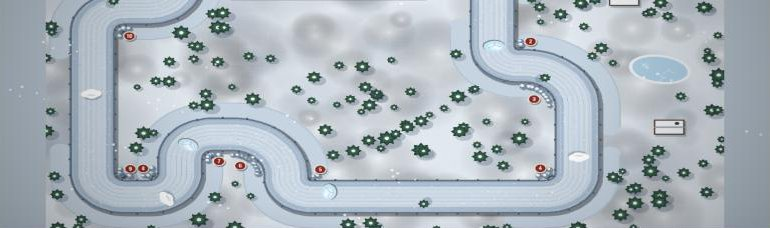
\includegraphics[width=.48\linewidth]{img/nieve.jpg}\hfill
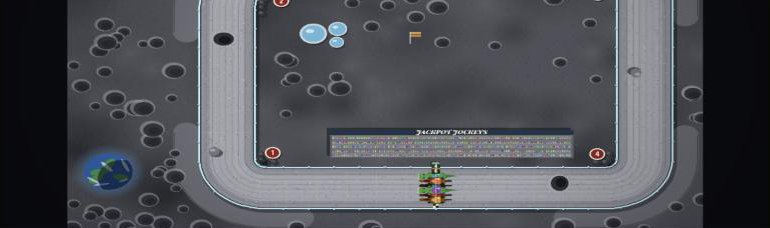
\includegraphics[width=.48\linewidth]{img/luna.jpg}\\[6pt]
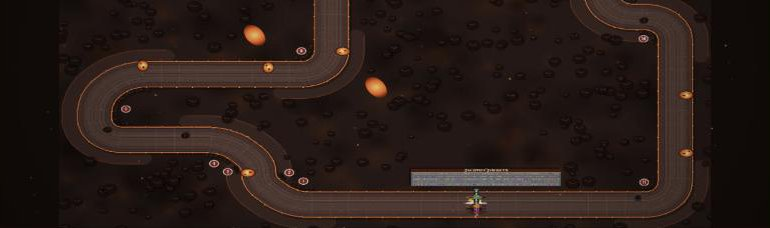
\includegraphics[width=.48\linewidth]{img/volcan.jpg}\hfill
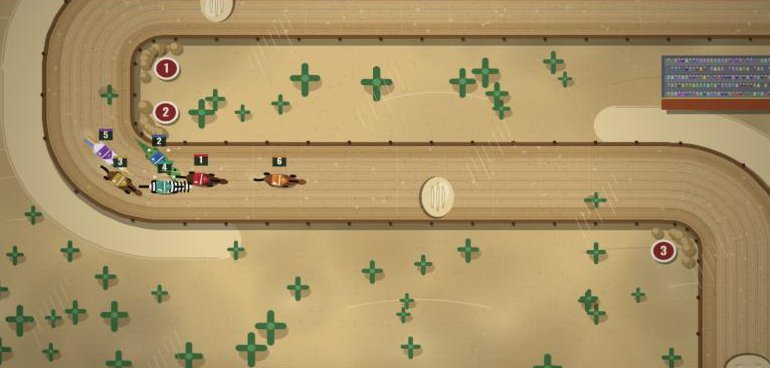
\includegraphics[width=.48\linewidth]{img/desierto.jpg}\\[6pt]
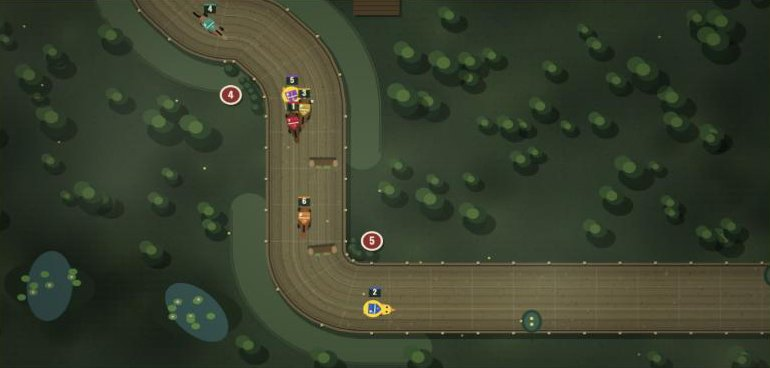
\includegraphics[width=.48\linewidth]{img/pantano.jpg}
\caption{Nieve, Luna, Volcán, Desierto y Pantano en la pantalla del juego.}
\end{figure}

\subsection{Obstáculos}
Cada mundo tiene obstáculos propios. Se colocan $\operatorname{round}(L/380)$ por pista, donde $L$ es el largo de la vuelta en píxeles, y el tipo se sortea con las probabilidades del mundo.

\begin{table}[h]
\centering
\begin{tabular}{llccl}
\toprule
Mundo & Obstáculo & Prob. & Radio & Efecto \\
\midrule
Hipódromo & Valla & .65 & 14 & Se salta; si no, tropieza \\
 & Barro & .35 & 22 & Se salta; si no, frena: $\times 0.55$ \\
Nieve & Pino & .35 & 13 & Sólido: no se salta, siempre tropieza \\
 & Hielo & .35 & 26 & Se salta; si no, el giro $\times 0.15$ \\
 & Nevada & .30 & 24 & Se salta; si no, frena: $\times 0.6$ \\
Luna & Roca & .50 & 13 & Se salta; si no, tropieza \\
 & Cráter & .50 & 14 & Se salta; si no, aturdido $0.8$ s. A un lado \\
Volcán & Lava & .40 & 22 & Se salta con $v \ge 8$; si no, al centro: $1.2$ s y salida \\
 & Géiser & .40 & 20 & Ciclo $150$ ticks, activo $45$: aturde $0.9$ s, también en el aire \\
 & Basalto & .20 & 14 & Se salta con $v \ge 8$; si no, tropieza \\
Desierto & Cactus & .35 & 12 & Sólido: no se salta, siempre tropieza \\
 & Arena & .35 & 28 & Se salta; si no, frena: $\times 0.65$ \\
 & Remolino & .30 & 24 & Gira $\pm 0.14$ rad/tick y frena $\times 0.85$, también en el aire \\
Pantano & Tronco & .25 & 16 & Se salta con $v \ge 7$ \\
 & Ciénaga & .20 & 26 & Se salta; si no, frena: $\times 0.45$ \\
 & Caimán & .55 & 18 & Ciclo $120$ ticks, activo $30$: aturde $1.1$ s, también en el aire \\
\bottomrule
\end{tabular}
\caption{Los 16 obstáculos.}
\end{table}

\begin{table}[h]
\centering
\begin{tabular}{lcccccc}
\toprule
Clase & lento & resbalón & desvío & hoyo & quema & ciclo \\
\midrule
Peligro percibido & 0.3 & 0.5 & 0.5 & 0.8 & 1 & 1 (0.2 apagado) \\
\bottomrule
\end{tabular}
\caption{Entrada 14 de la red según la clase de obstáculo que tiene adelante.}
\label{tab:peligro}
\end{table}

Un obstáculo de ciclo con fase $\varphi_o$ está activo en el tick $t$ si
\begin{equation}
(t + \varphi_o) \bmod P < D_a,
\end{equation}
con periodo $P$ y duración activa $D_a$. El sensor avisa desde 30 ticks antes de que se active: durante ese margen percibe peligro 1 aunque el obstáculo todavía no haga daño, así que la red puede anticiparlo.

\section{La física de cada tick}
La simulación corre a 30 ticks por segundo de juego. Sea $(x_t, y_t)$ la posición, $\theta_t$ la cabeza, $\phi_t$ la dirección real de avance y $v_t$ la velocidad. En cada tick, con $f$ la forma (hándicap por forma del día) y $a$ la agilidad:

\paragraph{Giro.} Con $\kappa = 0.15$ en hielo y $\kappa = 1$ en otro caso,
\begin{equation}
\theta_{t+1} = \theta_t + 0.08\, s\, a\, \kappa + \delta_{\text{remolino}}.
\end{equation}

\paragraph{Velocidad.} El objetivo depende del acelerador; $B$ es el producto de los efectos activos (turbo $1.5$, furia $1.15$, zanahoria $1.35$):
\begin{equation}
v^{*} = \left(3 + 3(g+1)\right) f\, V_w\, B, \qquad v^{*} \in \left(3,\ 9\right) f\, V_w\, B,
\end{equation}
\begin{equation}
v_{t+1} = v_t + I_w \left(v^{*} - v_t\right).
\end{equation}
Con $I_w = 1$ la velocidad cambia al instante, como en el hipódromo; en la Luna, con $I_w = 0.08$, tarda muchos ticks en subir o bajar. Pisar algo que frena con factor $\beta$ da
\begin{equation}
v \leftarrow \begin{cases} \beta\, v & \text{si } I_w = 1,\\ \left(1 - 0.15\,(1-\beta)\right) v & \text{si } I_w < 1. \end{cases}
\end{equation}
La segunda rama existe porque, con inercia, el frenazo se aplica en cada tick y se acumula.

\paragraph{Derrape.} El caballo no avanza hacia donde mira, sino hacia una dirección que persigue a la cabeza:
\begin{equation}
\phi_{t+1} = \phi_t + A_w \operatorname{wrap}\!\left(\theta_{t+1} - \phi_t\right), \qquad \operatorname{wrap}(\alpha) = \operatorname{atan2}(\sin\alpha, \cos\alpha).
\end{equation}
Es un filtro de primer orden: $A_w = 1$ no derrapa; con $A_w = 0.3$ (nieve) le toma varios ticks alinearse, y en las curvas se abre.

\paragraph{Viento.} Sopla en una dirección fija $\psi$ de cada pista, con una fuerza que oscila:
\begin{equation}
w(t) = U_w \sin\!\left(\frac{t}{48} + \rho\right),
\end{equation}
\begin{equation}
\begin{pmatrix} x_{t+1} \\ y_{t+1} \end{pmatrix} = \begin{pmatrix} x_t \\ y_t \end{pmatrix} + v_{t+1}\begin{pmatrix} \cos\phi_{t+1} \\ \sin\phi_{t+1} \end{pmatrix} + w(t)\begin{pmatrix} \cos\psi \\ \sin\psi \end{pmatrix}.
\end{equation}
La red percibe la componente lateral: $\operatorname{clip}\!\left(w(t)\sin(\psi - \theta)/U_w,\ -1,\ 1\right)$.

\paragraph{Sensores.} Cada rayo llega hasta $180\,C_w$ píxeles y se normaliza siempre con 180. Por eso, en el volcán, ningún rayo marca más de $0.55$: la ceniza acorta la vista y la red lo nota.

\paragraph{Saltos y esquives.} El salto es automático: al llegar a un obstáculo saltable, salta si $v \ge S_o$, donde $S_o$ es el umbral propio del obstáculo o, si no tiene, $S_w$. La red solo decide cuánto gira y cuánto corre, así que elegir entre saltar y esquivar es elegir entre llegar rápido o rodearlo. En las vallas, rocas, basalto y troncos, si no alcanza la velocidad queda aturdido $0.8$ s; en el barro, el hielo, la nieve, los cráteres, la lava, la arena y la ciénaga los pisa y hacen su efecto. Queda $T_w$ ticks en el aire, sin chocar.

Pino y cactus son sólidos: no se saltan. Géiser, remolino y caimán alcanzan también al que va en el aire (\texttt{atrapa}): la mordida o el chorro lo detienen y termina el salto. Un caimán o un géiser apagados no hacen nada, y se puede pasar por encima o a través de ellos. Se cuenta un esquive cuando un obstáculo queda atrás después de pasar a menos de $r + 30$ px, sin tocarlo a $r + 6$ px ni saltarlo.

\paragraph{Salirse.} Fuera de la pista, el jinete lo devuelve al centro en el punto de mayor avance y pierde $1.2$ s.

\paragraph{Choques.} Dos caballos chocan a menos de 18 px. Con $\hat u$ el vector unitario de uno hacia el otro y $P$ su fuerza, el empuje de cada uno es
\begin{equation}
p_a = v_a P_a \left(\cos\theta_a\, \hat u_x + \sin\theta_a\, \hat u_y\right).
\end{equation}
El de mayor $p$ embiste si $p \ge 1.5$ (con un enfriamiento de $0.8/P$ segundos): la víctima queda aturdida $0.6$ s ($1.2$ s si el atacante tiene furia) y desviada al azar hasta $\pm 0.4$ rad; el atacante gana medio segundo de turbo.

\section{Entrenar para toda la aleatoriedad}
Esta sección describe la neuroevolución con la que se entrenaron los perceptrones, de los que nacen los potros. Las GRU de la casa se entrenaron como explica la sección de experimentos; desde entonces, la evolución solo las afina durante la partida.
\subsection{Aptitud}
Tras correr, un caballo recibe
\begin{equation}
F = D + (T_{\max} - t_{\text{fin}}) + 5(J + Q) - 15E - c_s C + H\min(G, 8) - c_r R + P b - 40M,
\end{equation}
donde $D$ es el avance en puntos de trazado, $t_{\text{fin}}$ el tick de llegada (el segundo término vale cero si no termina), $J$ los saltos, $Q$ los esquives, que valen lo mismo, $E$ los tropiezos, $C$ las salidas, $G$ las embestidas dadas, $R$ las recibidas, $b$ los rivales que deja atrás y $M$ los obstáculos pisados.

\begin{table}[h]
\centering
\begin{tabular}{lcccccc}
\toprule
Cerebros & $H$ & $c_s$ & $c_r$ & $P$ & Velocidad al entrenar & Generaciones \\
\midrule
Corredor & 0 & 40 & 10 & 100 & 1.0 & 300 \\
Pícaro (bravo 60) & 60 & 60 & 20 & 100 & 1.0 & 300 \\
Bravo (bravo 100) & 100 & 60 & 20 & 150 & 1.2 & 250 \\
Muy bravo (bravo 150) & 150 & 60 & 20 & 180 & 1.2 & 250 \\
\bottomrule
\end{tabular}
\caption{Lo único que separa a las personalidades es cuánto se les premia embestir. Los valores de generaciones corresponden a la última ronda; cada ronda arranca de la anterior.}
\end{table}

\subsection{Evolución}
No hay gradientes ni aprendizaje durante la carrera. Con parámetros $\Theta \in \mathbb{R}^{199}$, en cada generación:
\begin{enumerate}
\item Se generan pistas nuevas, una por mundo, y la población de 36 corre en grupos de 6 sorteados.
\item Se promedia $F$ entre pistas y se ordena la población.
\item Pasan intactos los 8 mejores (elitismo), y los otros 28 son hijos mutados de un padre al azar entre ellos:
\begin{equation}
\Theta' = \Theta + \sigma\,\varepsilon, \qquad \varepsilon \sim \mathcal{N}(0, I), \qquad \sigma \sim \mathcal{U}[0.02,\ 0.15].
\end{equation}
\end{enumerate}
Como cada generación ve seis mundos y pistas distintas, un cerebro especializado en uno solo no sobrevive: lo que se selecciona es generalizar. Al final se eligen los 3 mejores en 18 pistas nuevas ($3$ tamaños $\times\ 6$ mundos). Los bravos entrenan contra corredores ya entrenados. Una ronda adicional de los bravos forzó el volcán en cada generación, porque ahí se seguían quemando.

\begin{figure}[h]
\centering
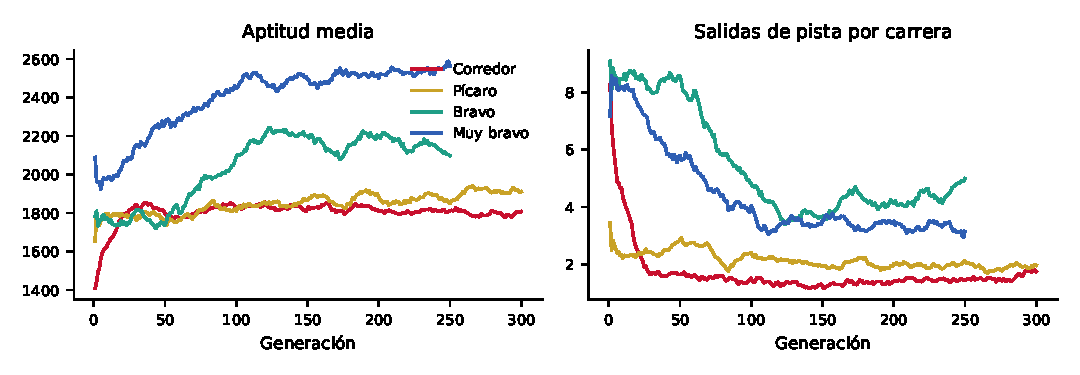
\includegraphics[width=\linewidth]{img/convergencia.pdf}
\caption{Aptitud media y salidas de pista por generación, tal como quedaron en \texttt{logs/}.}
\end{figure}

\subsection{Velocidad de cada personalidad}
Cada caballo $i$ corre con un multiplicador $h_i$. En carrera, $f = h_i\, u$, con forma del día $u \sim \mathcal{U}[0.93,\ 1.07]$. Con las GRU se fija a mano: $1$ al corredor, $0.98$ al pícaro, $1$ al bravo y $1.09$ al muy bravo. No se iguala la tasa de victorias, porque se comprobó que eso borra las personalidades (sección de experimentos); las diferencias que quedan las absorben las cuotas. \texttt{calibrar.js} conserva el ajuste automático de antes para quien quiera usarlo, y con 0 iteraciones solo mide las cuotas por mundo:
\begin{equation}
h_i \leftarrow h_i \left(\frac{1/n}{\max(p_i,\ 0.01)}\right)^{0.07},
\end{equation}
tras lo cual se normalizan a media 1 y se recortan a $[0.7,\ 1.25]$. Los potros corren con $0.985$ el corredor y $1.10$ el bravo, ajustados para que sigan llegando al podio con las redes nuevas.

\section{Aprender durante la partida}
\subsection{Caballos de la casa}
Después de cada carrera, los caballos de la casa repasan en segundo plano mientras el juego está abierto. Con $n_X$ los errores que cometió en esa carrera, el castigo de cada error crece con $\text{peor}(n) = 1 + \min(n, 2)$:
\begin{equation}
\begin{split}
F_{\text{lección}} = {} & D + (T_{\max} - t_{\text{fin}}) + 5J + H_k \min(G, 8) + 300\,b \\
& - 15\,\text{peor}(n_E)\,E - 40\,\text{peor}(n_C)\,C - 10\,\text{peor}(n_R)\,R - 40\,\text{peor}(n_M)\,M,
\end{split}
\end{equation}
con $H_k = 0, 60, 100, 150$ según la personalidad. Son 30 generaciones, población 18 y élite 5. La mutación usa $\sigma \in [0.02,\ 0.1]$ multiplicado por $0.05$, porque una GRU se rompe con mutaciones normales (sección de experimentos); el mundo de esa carrera se fuerza en una de las tres pistas de cada generación.

\paragraph{Examen pareado.} Un caballo puede parecer mejor por pura suerte, así que el cambio se conserva solo si pasa un examen en 36 pistas nuevas, recorridas por el caballo viejo y el nuevo con la misma semilla de azar. Con $\Delta_j$ la diferencia de rivales vencidos en la pista $j$:
\begin{equation}
\bar\Delta = \frac{1}{36}\sum_{j}\Delta_j, \qquad \mathrm{SE} = \frac{\operatorname{sd}(\Delta)}{\sqrt{36}},
\end{equation}
\begin{equation}
\text{se acepta} \iff \bar\Delta > 0 \ \wedge\ \bar\Delta > \tfrac{1}{2}\mathrm{SE} \ \wedge\ \bar G_{\text{después}} \ge 0.8\, \bar G_{\text{antes}}.
\end{equation}
La última condición, para los que embisten, impide que pierdan su personalidad. Es un criterio poco exigente (medio error estándar): deja pasar algunas falsas mejoras a cambio de no desperdiciar las reales.

\paragraph{Entrenan el cuerpo.} Además, cada línea de la casa entrena el cuerpo cada 5 carreras que corre, como un potro, hasta 6 veces. Usa los mismos pasos que los potros (velocidad $+0.015$, giro $+0.05$, fuerza $+0.1$, con los mismos topes) en un orden fijo para cada personalidad:
\begin{center}\footnotesize
\begin{tabular}{ll}
\toprule
Corredor & velocidad, giro, velocidad, giro, velocidad, velocidad \\
Pícaro & giro, velocidad, giro, velocidad, velocidad, fuerza \\
Bravo & fuerza, velocidad, fuerza, velocidad, giro, velocidad \\
Muy bravo & giro, fuerza, giro, velocidad, giro, fuerza \\
\bottomrule
\end{tabular}
\end{center}
A diferencia del potro, el cerebro no se reentrena: así no pierde su forma de correr, y el cuerpo nuevo no necesita examen porque solo puede ayudar. El cuerpo se guarda junto a lo aprendido, entra en las lecciones (que se repasan con ese cuerpo) y en el cálculo de $\epsilon_i$, así que las cuotas lo siguen. Con 8 líneas y 6 caballos por carrera, cada línea corre unas 3 de cada 4 carreras: el primer entrenamiento llega hacia la carrera 7 y el último hacia la 40. El narrador lo anuncia.

\subsection{Potros de los jugadores}
Los potros siguen naciendo con perceptrones, los del corredor o el bravo anteriores, y los que ya existían conservan su cerebro. Falta probar si una GRU entrenaría igual de bien. Su entrenamiento no cambió. Cada entrenamiento sube un rasgo del cuerpo (velocidad $+0.015$ hasta $0.06$, giro $+0.05$ hasta $0.2$, fuerza $+0.1$ hasta $0.4$), reentrena el cerebro 60 generaciones con ese cuerpo y lo examina igual, contra el caballo de antes. El cerebro nuevo se conserva si $\bar\Delta > \mathrm{SE}/2$ en el rasgo y no pierde más de $0.3$ rivales vencidos por carrera. Cuesta una carrera: mientras entrena, el potro no compite.

\section{Las cuotas}
\subsection{Probabilidad}
La probabilidad parte de lo esperado de cada caballo $i$ en el mundo $w$, según lo aprendido $\epsilon_i$ y la ventaja de su personalidad $k$, $e_{w,k}$:
\begin{equation}
\pi^{0}_i = \frac{\epsilon_i\, e_{w,k_i}}{\sum_j \epsilon_j\, e_{w,k_j}}.
\end{equation}
Las victorias reales en el juego corrigen ese punto de partida. Tras cada carrera, con $g_i = 1$ si ganó y $0.98$ de memoria, que hace pesar las últimas 50 carreras más o menos:
\begin{equation}
W_i \leftarrow 0.98\, W_i + g_i, \qquad E_i \leftarrow 0.98\, E_i + \pi^{0}_i.
\end{equation}
La probabilidad con que se calculan las cuotas es
\begin{equation}
\pi_i = \frac{\pi^{0}_i\, \dfrac{W_i + 5}{E_i + 5}}{\sum_j \pi^{0}_j\, \dfrac{W_j + 5}{E_j + 5}}.
\end{equation}
El 5 equivale a cinco victorias esperadas de duda: al principio casi no se mueve, porque pocas carreras son azar, y un solo triunfo inesperado multiplica el peso del caballo por unos $1.16$. $W_i$ y $E_i$ se guardan por caballo en \texttt{victorias.json} entre partidas. En la primera carrera de cada partida los caballos de la casa pagan igual, aunque esa carrera sí se cuenta. Reemplaza al sistema anterior, que usaba un rating según el puesto y solo dentro de cada partida.

\paragraph{Ventaja por mundo.} Con $V_k$ las victorias de la personalidad $k$ en $R = 2000$ carreras simuladas en ese mundo, $m_k$ los caballos que la tienen y suavizado $\lambda = 15$:
\begin{equation}
e_{w,k} = \frac{V_k + \lambda\, m_k}{R + \lambda\, n} \cdot \frac{n}{m_k}.
\end{equation}

\paragraph{Ventaja aprendida.} Con $w_i$ victorias en $R = 600$ carreras simuladas y suavizado 5:
\begin{equation}
\epsilon_i = \frac{w_i + 5}{R + 5n}\, n.
\end{equation}
Un potro entrenado multiplica su peso por $\exp(20\,\text{vel} + 4\,\text{giro})$.

\begin{table}[h]
\centering
\begin{tabular}{lccccl}
\toprule
Mundo & Corredor & Pícaro & Bravo & Muy bravo & Suele ganar \\
\midrule
Hipódromo & 0.792 & 1.093 & 1.059 & 1.055 & Pícaro \\
Nieve & 0.922 & 1.301 & 1.042 & 0.734 & Pícaro \\
Luna & 1.074 & 1.443 & 0.874 & 0.601 & Pícaro \\
Volcán & 1.452 & 0.881 & 0.994 & 0.673 & Corredor \\
Desierto & 1.304 & 0.967 & 1.007 & 0.721 & Corredor \\
Pantano & 1.042 & 0.994 & 1.003 & 0.962 & Corredor \\
\bottomrule
\end{tabular}
\caption{$e_{w,k}$ medido con 400 carreras por mundo, con las GRU adoptadas, con un error de unos $0.2$. 1 es ``gana lo que le toca''. Nadie programó estas diferencias: en la Luna, por ejemplo, el muy bravo rinde mucho menos.}
\end{table}

\subsection{De la probabilidad a la cuota}
Para las combinadas se usa la fórmula de Harville:
\begin{equation}
P(i_1, i_2, \dots, i_m \text{ en ese orden}) = \prod_{\ell=1}^{m} \frac{\pi_{i_\ell}}{1 - \sum_{u<\ell} \pi_{i_u}}.
\end{equation}
Por ejemplo, $P(i \text{ queda 1º o 2º}) = \pi_i + \sum_{j\ne i} \pi_j\pi_i/(1-\pi_j)$. La cuota es
\begin{equation}
O = \operatorname{clip}\!\left(\min\!\left(\frac{\tau_c}{P},\ 1.2\,\frac{\tau_c}{P_{\text{iguales}}}\right),\ 1.05,\ 5000\right),
\end{equation}
donde $\tau_c$ es el factor de pago en la carrera $c$, que sube linealmente desde su valor inicial $\tau^0$ hasta $0.8$:
\begin{equation}
\tau_c = \tau^0 + (0.8 - \tau^0)\min\!\left(1,\ \frac{c-1}{4}\right).
\end{equation}
El valor esperado de apostar una ficha con cuota $O$ a algo de probabilidad real $P^{*}$ es $O P^{*}$; si la casa estima bien, vale $\tau_c$. Es decir: desde la carrera 5, por cada ficha apostada se devuelven 0.8 en promedio. En la carrera 1 ``Que gane'' paga x2 en todos, y las primeras carreras son deliberadamente generosas.

\subsection{Comisión del dueño}
Si gana un potro con dueño, además de su premio, el dueño recibe el 20\,\% de lo que ganó la casa con las apuestas de esa carrera:
\begin{equation}
\text{comisión} = \left\lfloor 0.2\, \max\!\left(0,\ \textstyle\sum \text{apostado} - \sum \text{pagado}\right) \right\rfloor.
\end{equation}

\section{Resultados medidos}
Antes de entrenar por mundo, en el volcán el 76\,\% de los caballos no llegaba a la meta y había 31 salidas por carrera. Con las GRU, ningún caballo dejó de llegar en ningún mundo.

\begin{table}[h]
\centering
\begin{tabular}{lcccccc}
\toprule
Mundo & Tiempo (s) & No llega & Salidas & Tropiezos & Pisados & Embestidas \\
\midrule
Hipódromo & 29.2 & 0\,\% & 1.0 & 0.0 & 0.1 & 2.1 \\
Nieve & 32.3 & 0\,\% & 1.2 & 0.9 & 0.2 & 2.1 \\
Luna & 29.9 & 0\,\% & 1.3 & 0.2 & 0.1 & 2.0 \\
Volcán & 31.4 & 0\,\% & 1.4 & 0.3 & 0.4 & 2.6 \\
Desierto & 31.4 & 0\,\% & 1.3 & 1.1 & 2.9 & 2.3 \\
Pantano & 31.1 & 0\,\% & 0.9 & 0.2 & 0.2 & 2.3 \\
\bottomrule
\end{tabular}
\caption{Promedio por caballo y carrera en 100 carreras de cada mundo, con las GRU adoptadas. Antes el rango de tiempos era de $30.7$ a $37.8$ s y en el desierto se pisaban $7.9$ obstáculos: se pisan menos, pero los mundos se distinguen menos por el tiempo.}
\end{table}

\begin{table}[h]
\centering
\begin{tabular}{lcc}
\toprule
Salidas por carrera & Primeras 20 gen. & Últimas 20 gen. \\
\midrule
Corredor & 3.15 & 1.74 \\
Pícaro & 2.38 & 1.97 \\
Bravo & 8.56 & 4.90 \\
Muy bravo & 7.77 & 3.07 \\
\bottomrule
\end{tabular}
\caption{Mejora durante la evolución de los perceptrones: primeras y últimas 20 generaciones de los registros.}
\end{table}

\paragraph{La casa.} Con las redes adoptadas, ver la subsección \emph{Sin maestro} de Experimentos: en 11000 carreras ninguna estrategia pasó de $0.84$ por ficha. Con las redes anteriores se simularon 4000 carreras en partidas de 10, con las cuotas por victorias y sin poderes ni potros. Se probaron seis tipos de apuesta, cada uno apostando a todo, al favorito y a lo que más paga. Desde la carrera 5, lo mejor fue el podio apostando a todo, con $0.78$ por ficha, y apostar a lo que más paga no pasó de $0.68$. En las carreras 1 a 4, nada pasó de $0.66$. No se repitió la prueba de apostar sabiendo el mundo, y no se puso a prueba a un jugador que aproveche el retraso del historial. El sistema anterior llegaba a $0.86$--$0.88$ sin mirar el mundo y a $1.00$--$1.13$ sabiéndolo.

\paragraph{Aprendizaje por carrera con las GRU.} Con las redes adoptadas, de 12 lecciones pasaron el examen 4; con las anteriores, 9. El examen es poco exigente. Tardan unos 23 s cada una, frente a 13 s de un perceptrón. No se midió todavía cuánto ganan de más tras varias lecciones.

\paragraph{Aprendizaje por carrera con los perceptrones anteriores.} Cada caballo tomó 8 lecciones por separado, en mundos al azar y contra los otros cinco sin aprender. Luego se comparó antes y después en 600 carreras de todos los mundos con las mismas semillas.

\begin{table}[h]
\centering
\begin{tabular}{lcccc}
\toprule
Caballo & Aceptadas & Gana (\%) & Puesto medio & Salidas \\
\midrule
Don Galope & 1/8 & $16.3 \to 18.3$ & $3.15 \to 3.21$ & $1.08 \to 1.14$ \\
Herradura Loca & 1/8 & $16.3 \to 30.7$ & $4.01 \to 3.40$ & $2.94 \to 3.25$ \\
Sir Relincho & 0/8 & $17.7 \to 17.7$ & $3.26 \to 3.26$ & $1.00 \to 1.00$ \\
Patas de Trueno & 4/8 & $17.5 \to 17.5$ & $3.68 \to 3.56$ & $2.03 \to 2.44$ \\
Pura Sangre Fría & 2/8 & $16.0 \to 15.8$ & $3.35 \to 3.32$ & $1.07 \to 1.12$ \\
Pancho Trotes & 2/8 & $18.5 \to 18.8$ & $3.35 \to 3.29$ & $1.57 \to 1.55$ \\
\bottomrule
\end{tabular}
\caption{Antes y después de 8 lecciones. Con 600 carreras, el error estándar de cada porcentaje de victorias es de unos 1.5 puntos.}
\label{tab:lecciones}
\end{table}

Herradura Loca es la única mejora clara, y es la que más margen tenía, porque era la de peor puesto medio. Una sola lección aceptada le bastó; también se sale un poco más. Cuando un caballo mejora así, $\epsilon_i$ baja sus cuotas para que apostarle no le gane a la casa. Lo aprendido por esas redes no pasa a las GRU: se guardaba en otro archivo, que ya no se lee.

\section{Jugar desde otra red}
La dirección del QR es la de la WiFi, así que un celular con datos móviles o en otra red no llega al juego. Debajo del QR, el botón \emph{Abrir a internet} abre un túnel temporal de Cloudflare (\texttt{cloudflared}, gratis y sin cuenta), que da un enlace público \texttt{https://…trycloudflare.com} hacia el puerto del juego. El QR se cambia solo a ese enlace, y todas las pantallas de la sala ven en vivo el estado: descargando, abriendo, listo o error. Si \texttt{cloudflared} no está instalado, el juego descarga una sola vez la versión oficial de Cloudflare en GitHub para Mac, Windows o Linux y la guarda junto a sus datos. El túnel se cierra con el botón o al cerrar el juego; nada queda corriendo. Lo mismo se hace desde el menú de la app o con \texttt{npm run compartir}. Todo vive en \texttt{tunel.js}.

\paragraph{Prueba.} En el Mac, con datos temporales, la descarga de \texttt{cloudflared} (39 MB) tardó $1.1$ s y el túnel quedó listo en $3.7$ a $5.1$ s; se registró en el centro de datos de Bogotá y, al cerrarlo, no quedó ningún proceso. El enlace no se pudo abrir desde el mismo Mac: la red de la casa no resuelve los subdominios de \texttt{trycloudflare.com} y, resolviéndolos por fuera, la conexión segura no termina; la página general de \texttt{api.trycloudflare.com} sí responde. La explicación probable, no comprobada, es un filtro de la red o del proveedor. Un lector de páginas externo recibió un 403 del borde de Cloudflare, que suele rechazar a los robots, así que tampoco confirma que un celular entre. Falta probarlo con un celular real con datos móviles.

\section{El video tutorial}
La primera vez que se abre el juego en un equipo sale un video con voz, de unos dos minutos, que explica cómo entrar, apostar, las personalidades, los mundos, los poderes, los potros, la mafia y las peñas. Se salta con un botón o con Enter, y se vuelve a ver con la tecla V o desde la pantalla de inicio. Se graba con el juego real desde \texttt{video/grabar.js}, con un guion en \texttt{video/guion.js}; lo que se ve hay que volver a grabarlo si cambia el juego. El video actual dura 2:22, se grabó con las redes adoptadas y ya explica las personalidades al azar, los saltos y que los caimanes muerden aunque se salte. Se revisaron sus escenas y que la pista de audio decodifica, pero nadie ha escuchado la voz de esta versión de principio a fin.

\section{Experimentos}
Cada idea se prueba primero en una copia aparte, sin tocar el juego, y solo se adopta si los números la justifican. Aquí quedan también las que no funcionaron. Salvo que se diga otra cosa, ``tropiezos'', ``salidas'' y ``pisadas'' son por caballo y por carrera. Las pruebas usan pocas carreras comparadas con el ruido del juego, así que las diferencias pequeñas no significan nada.

\subsection{Castigar más los tropiezos: descartado}
Se reentrenó a todos con $100E$ en lugar de $15E$ en la aptitud y se midieron 200 carreras por mundo. En la Luna los tropiezos pasaron de $7.9$ a $7.5$, los demás mundos quedaron iguales, y en el volcán las salidas subieron de $3.6$ a $4.3$. Castigar más no enseña a esquivar si no hay espacio para hacerlo.

\subsection{Cráteres más pequeños y a un lado: adoptado}
El 99\,\% de los tropiezos de la Luna ocurría en cráteres. Con los mismos caballos, sin reentrenar:

\begin{table}[h]\centering
\begin{tabular}{lc}
\toprule
Cráter & Tropiezos en la Luna \\
\midrule
Radio 22, cerca del centro (antes) & 7.87 \\
Radio 14, cerca del centro & 5.20 \\
Radio 22, a un lado & 2.79 \\
Radio 14, a un lado (adoptado) & 1.31 \\
\bottomrule
\end{tabular}
\caption{Moverlos a un lado pesa más que achicarlos. 200 carreras.}
\end{table}

\subsection{Saltar barro, nieve y cráteres: adoptado}
Los obstáculos marcados como saltables se saltan si el caballo llega con $v \ge v_{\text{salto}}$ del mundo; si no, se pisan y hacen su efecto. En el hipódromo las pisadas bajaron de $5.4$ a $0.2$, en la nieve de $11.7$ a $6.8$ (el hielo no se salta) y en la Luna de $1.3$ a $0.0$, con los tropiezos de $1.4$ a $0.1$. El precio es que, con buena velocidad, esos obstáculos casi no afectan quién gana.

\subsection{Más caimanes en el pantano: adoptado}
El caimán pasó de $.30$ a $.55$ de los obstáculos, unos $5.5$ por pista en vez de unos $3$. La carrera casi no cambió: los tropiezos fueron de $0.6$ a $0.7$. Es sobre todo un cambio visual; para que muerdan más habría que dejarlos activos más tiempo o acercarlos al centro.

\subsection{Cruzar caballos: viable, sin construir}
Se cruzaron pares de caballos de tres formas y cada hijo corrió 240 carreras en los seis mundos contra los mismos rivales, con la misma forma física para comparar solo el cerebro.

\begin{table}[h]\centering
\begin{tabular}{lcc}
\toprule
Don Galope $\times$ Patas de Trueno & Puesto medio & Salidas \\
\midrule
Padres & 2.26 y 4.17 & 1.5 y 1.7 \\
Promedio de los pesos & 2.63 & 1.4 \\
Una capa de cada padre & 3.70 & 2.1 \\
Mezcla al azar de cada peso & 5.91 & 7.9 \\
\bottomrule
\end{tabular}
\caption{Ejemplo: el promedio es la única forma que no produjo ningún hijo roto.}
\end{table}

Los rasgos se heredan: Don Galope ($2.9$ embestidas) $\times$ Herradura Loca ($5.0$) da un hijo promedio con $3.7$. Pero ningún hijo superó con claridad a su mejor padre. Don Galope, Sir Relincho y Pura Sangre Fría tienen cerebros casi idénticos (distancia media por peso de $0.36$ a $0.39$, contra $7$ a $11$ con los bravos), así que cruzarlos da casi el mismo caballo. El diseño pendiente es sin géneros: promedio más una mutación pequeña, varios potros y queda el mejor de un examen.

\subsection{El caballo de heurística: las redes no están en el límite}
Para saber cuánto margen queda se programó un caballo sin red. Conoce toda la pista y las reglas: apunta al punto más lejano que alcanza en línea recta sin salirse ni pisar lo que no se salta, y ensaya $14$ ticks hacia adelante para elegir la mayor velocidad que no lo saca de la pista. Un primer intento con línea de carrera precalculada salió peor y se descartó.

\begin{table}[h]\centering
\begin{tabular}{lcccc}
\toprule
Mundo & \multicolumn{2}{c}{Tiempo solo (s)} & \multicolumn{2}{c}{Salidas} \\
 & Heurística & Don Galope & Heurística & Don Galope \\
\midrule
Hipódromo & 27.0 & 29.0 & 0.00 & 0.88 \\
Nieve & 31.5 & 33.7 & 0.10 & 1.52 \\
Luna & 27.0 & 29.0 & 0.07 & 1.18 \\
Volcán & 29.7 & 32.6 & 0.83 & 2.45 \\
Desierto & 29.9 & 31.1 & 0.18 & 0.88 \\
Pantano & 29.2 & 30.3 & 0.00 & 0.78 \\
\bottomrule
\end{tabular}
\caption{60 carreras por mundo, corriendo solos.}
\end{table}

Contra los caballos de la casa, y sin hándicap a su favor, ganó entre el 39\,\% (pantano) y el 86\,\% (volcán) de 100 carreras por mundo. La comparación no es del todo justa, porque la heurística ve el mapa completo y la red solo sus sensores: es un techo, no una meta segura. No pelea ni esquiva rivales, y aún tropieza algo en nieve y volcán.

\subsection{Resistencia: sin adoptar}
Hoy el acelerador va a fondo el 95\,\% del tiempo porque no cuesta nada. Para que sea una decisión se añadió, solo en la copia, un aguante $a \in [0,1]$ y dos entradas a la red ($a$ y la fracción de carrera hecha), con el acelerador $g \in [0,1]$:
\begin{equation}
a \leftarrow a + \frac{1-g}{300} - \frac{g^2}{420}, \qquad v \leftarrow v \left(0.65 + 0.35 \min\!\left(1, \frac{a}{0.3}\right)\right).
\end{equation}
Ir a fondo agota en unos 14 s y con $g \approx 0.71$ el aguante no cambia.

\begin{table}[h]\centering
\begin{tabular}{lccc}
\toprule
240 carreras & Sin resistencia & Sin reentrenar & Reentrenados \\
\midrule
Cambios de líder por carrera & 2.07 & 3.53 & 2.93 \\
El líder a mitad de carrera gana & 75\,\% & 44\,\% & 52\,\% \\
Tiempo medio (s) & 34.5 & 40.9 & 39.9 \\
Acelerador a fondo & 95\,\% & 93\,\% & 94\,\% \\
\bottomrule
\end{tabular}
\caption{Primera ronda: más disputa, pero por agotamiento y no por estrategia.}
\end{table}

Los corredores siguieron al 100\,\% de acelerador y llegaron sin fuerzas. Dosificar sí conviene: la misma red con el acelerador limitado a mano al 75\,\% baja de $37.6$ a $34.7$ s corriendo sola. El entrenamiento no lo encontró, probablemente porque el acelerador queda saturado por pesos muy grandes (sin comprobar).

En un segundo intento las redes arrancaron con el acelerador cerca de $78$\,\%: se redujeron los pesos de esa salida y se ajustó su sesgo. Así sí mantuvieron el ritmo:

\begin{table}[h]\centering
\begin{tabular}{lccc}
\toprule
240 carreras & Sin resistencia & Primer intento & Desde 78\,\% \\
\midrule
Acelerador a fondo & 95\,\% & 94\,\% & 6\,\% \\
Salidas & 1.64 & 1.44 & 0.81 \\
Tropiezos & 1.03 & 1.25 & 1.20 \\
Embestidas & 4.0 & 4.5 & 2.7 \\
Cambios de líder por carrera & 2.07 & 2.93 & 1.93 \\
El líder a mitad de carrera gana & 75\,\% & 52\,\% & 68\,\% \\
Tiempo medio (s) & 34.5 & 39.9 & 36.8 \\
\bottomrule
\end{tabular}
\caption{Corren dosificados y se salen menos, pero sin estrategia y sin más disputa.}
\end{table}

El acelerador casi no varía entre los cuartos de carrera (el corredor va al $80$\,\% en los cuatro) y llegan con aguante de sobra. El defecto parece estar en la regla: un ritmo fijo del $80$\,\% ya hace $34.7$ s, contra $34.5$ s de la heurística, así que variar no da premio. No se adoptó. Para que aparezca estrategia, apretar en ciertos momentos tendría que pagar, por ejemplo con el rebufo detrás de un rival. Tampoco se probó el currículo gradual de fatiga, porque su fin era despegar el acelerador y eso ya se logró. Falta medir aparte si correr menos a fondo baja las salidas por sí solo.

\subsection{Otras arquitecturas: sin ventaja medible}
Se entrenaron corredores con el mismo presupuesto (200 generaciones, población 36, los seis mundos, sin resistencia), y se midieron en las mismas pistas: 120 carreras solos y 180 contra los mismos rivales de la casa. Las variantes con pesos en cero arrancan exactamente igual que la red actual, lo que se comprobó antes de entrenar. Cada una tiene pocas semillas, así que solo detecta diferencias grandes.

\begin{table}[h]\centering\small
\begin{tabular}{lccc}
\toprule
Variante & Tiempo solo (s) & Salidas & Gana contra la casa \\
\midrule
Red actual, sin reentrenar & 31.31 & 1.56 & 42\,\% \\
Red actual, reentrenada & 31.05 / 31.36 & 1.48 / 1.50 & 44 / 39\,\% \\
Sentidos: curva, derrape y velocidad & 31.25 / 30.98 & 1.49 / 1.46 & 36 / 32\,\% \\
Primera capa de 16 neuronas & 31.03 / 31.18 & 1.55 / 1.46 & 39 / 37\,\% \\
GRU de 4 añadida & 30.94 / 31.18 & 1.45 / 1.49 & 42 / 36\,\% \\
Sentidos y GRU de 4 & 31.11 / 30.96 & 1.48 / 1.49 & 39 / 41\,\% \\
Entradas de hace 4 y 8 ticks & 31.03 / 31.15 & 1.19 / 1.43 & 30 / 40\,\% \\
Mixta con GRU de 8, desde cero & 31.32 / 31.24 & 1.63 / 1.52 & 36 / 36\,\% \\
Red actual desde cero & 31.20 / 31.81 & 1.56 / 1.73 & 32 / 32\,\% \\
Red actual desde cero, 600 gen. & 31.09 / 31.51 & 1.51 / 1.59 & 37 / 28\,\% \\
GRU pura de 8 (666 pesos), 600 gen. & 31.06 / 31.84 / 31.71 & 1.35 / 0.73 / 1.63 & 38 / 34 / 28\,\% \\
\midrule
Heurística & 28.81 & 0.19 & 64\,\% \\
\bottomrule
\end{tabular}
\caption{Ninguna arquitectura se separa de la red actual, ni se acerca a la heurística.}
\end{table}

La distancia con la heurística parece estar en los errores. Con unas $1.3$ salidas de más a $1.2$ s y unos $0.9$ tropiezos de más a $0.8$ s se explican unos $2.3$ s, casi toda la diferencia; es una cuenta aproximada, no una medición directa. Que redes tan distintas, incluso desde cero, queden en el mismo punto apunta al entrenamiento o a la aptitud, no al modelo, aunque tampoco está comprobado. La hipótesis siguiente es que no aprenden a frenar antes de las curvas. Las pruebas son solo con corredores, y una red grande podría necesitar más generaciones.

\subsection{Imitar a la heurística con una GRU: sin adoptar en esa prueba}
Para separar si el freno es el entrenamiento o la red, se entrenaron redes con gradientes para copiar a la heurística, con DAgger: primero conduce la heurística; luego conduce la red, y en cada tick la heurística dice qué habría hecho. Hubo 10 rondas de 240 carreras, mitad solos y mitad con rivales, con el error cuadrático sobre giro y acelerador. La red entrenada en Python da el mismo resultado en el juego, con error menor que $10^{-6}$. Solo se entrenó el corredor, y de cada variante hay dos semillas.

\begin{table}[h]\centering\small
\begin{tabular}{lcccc}
\toprule
Variante & Tiempo solo (s) & Salidas & Pisadas & Gana contra la casa \\
\midrule
Red actual, con evolución & 31.31 & 1.56 & 3.8 & 42\,\% \\
Red actual, imitando & 32.29 / 32.12 & 1.63 / 1.64 & 3.8 / 3.3 & 28 / 27\,\% \\
GRU de 8 (666 pesos), imitando & 31.57 / 31.33 & 1.22 / 1.07 & 3.1 / 3.0 & 34 / 33\,\% \\
GRU de 32 (4962 pesos), imitando & 31.75 / 30.89 & 1.78 / 0.90 & 2.4 / 2.1 & 33 / 37\,\% \\
\midrule
Heurística & 28.81 & 0.19 & 0.9 & 64\,\% \\
\bottomrule
\end{tabular}
\caption{Con gradientes la GRU sí supera a la red sin memoria, pero aún no a la evolución en carrera.}
\end{table}

La mejor red, una GRU de 32, gana en unos mundos y pierde en otros frente a la red actual: hipódromo $28.8$ contra $30.1$ s, Luna $26.9$ contra $28.3$ y pantano $28.9$ contra $30.4$, pero desierto $31.3$ contra $30.7$ y volcán $34.8$ contra $33.8$; en nieve hace $34.7$ contra $34.5$. La otra semilla de la misma arquitectura salió mucho peor, así que el resultado no es estable. La pérdida se quedó en torno a $0.43$, lejos de copiar del todo: lo más probable es que con estos sensores la red no pueda deducir todo lo que la heurística ve en el mapa. Sin memoria, imitar salió peor que evolucionar, así que la imitación por sí sola no explica la mejora. Corrige la conclusión de la sección anterior: el método de entrenamiento sí cambia lo que aporta la memoria. No se adoptó porque gana menos contra la casa y costaría reentrenar a todos con gradientes, reescribir el entrenamiento durante la partida y guardar la memoria de cada caballo.

\subsection{Afinar la GRU con evolución: descartado en esa prueba}
La mejor GRU de 32 se afinó con la aptitud de carrera, 300 generaciones y tres semillas. La regla, fijada antes de empezar, era congelar las redes si no superaba a la red actual contra la casa.

\begin{table}[h]\centering
\begin{tabular}{lcccc}
\toprule
Variante & Tiempo solo (s) & Salidas & Volcán (s) & Gana contra la casa \\
\midrule
Red actual & 31.31 & 1.56 & 33.8 & 42\,\% \\
GRU imitando, sin afinar & 30.89 & 0.90 & 34.8 & 37\,\% \\
GRU afinada, semilla 1 & 33.00 & 2.82 & 45.3 & 23\,\% \\
GRU afinada, semilla 2 & 31.65 & 0.78 & 39.4 & 26\,\% \\
GRU afinada, semilla 3 & 32.10 & 1.32 & 37.6 & 12\,\% \\
\bottomrule
\end{tabular}
\caption{Afinar empeoró a la GRU en carrera; las tres semillas quedan por debajo.}
\end{table}

En la primera generación la población promedia entre $438$ y $845$ puntos, con $15$ a $20$ salidas por carrera, mientras el mejor individuo supera los $2200$: mutar una red de 4962 pesos entrenada con gradientes casi siempre la rompe. Es una explicación probable de por qué la evolución no la mejoró, no una comprobación. La decisión en ese momento fue congelar las redes. Solo se probó con el corredor. Después se decidió pasar a las GRU de todos modos, y bajar la mutación apoyó esta explicación (siguiente sección).

\subsection{Personalidades con GRU: adoptado}
Por decisión del dueño del juego, aunque la GRU del corredor no había superado a la red anterior contra la casa, los seis caballos pasaron a GRU de 32. El reto era conservar las personalidades, que antes salían de premiar las embestidas.

\paragraph{Maestro con personalidad.} La heurística anterior es el maestro y se le añadió un estilo que solo usa lo que la red también percibe: el corredor esquiva a un rival muy cercano; los demás buscan al rival más cercano si lo tienen a tiro, con distinto alcance, cono y acelerador mínimo, y el muy bravo no mira si se sale. Cada red imita con DAgger, en 10 rondas de 240 carreras, con velocidad al azar en torno a la de su personalidad.

\paragraph{Primer intento: fracasó.} Con personalidades que afectaban poco la conducta y mucha diferencia de velocidad ($0.92$ a $1.25$), las redes se distinguían, pero por la velocidad. Al igualar victorias con el hándicap, todas quedaron en torno a $1$ y las personalidades se borraron: entre $2.05$ y $2.31$ golpes para todas, y el corredor era el que más se salía ($1.68$). Con la velocidad distinta, en cambio, el muy bravo ganaba hasta el 56\,\% en pista larga. Esas redes se descartaron.

\paragraph{Segundo intento: adoptado.} Se endureció la conducta del maestro y las velocidades se acercaron. A igual velocidad, el maestro da $1.38$, $2.27$, $2.33$ y $2.43$ golpes, y $0.53$, $0.77$, $1.41$ y $2.67$ salidas. Se entrenaron 10 redes y se eligieron las seis del juego por sus resultados contra la casa anterior.

\begin{table}[h]\centering\small
\begin{tabular}{lcccccc}
\toprule
 & Podio & Golpes & Recibe & Salidas & Gana c/m/l (\%) \\
\midrule
Corredor, anterior & 57\,\% & 3.19 & 3.79 & 0.96 & 22 / 19 / 14 \\
Corredor, GRU & 56\,\% & 1.87 & 2.67 & 1.33 & 19 / 17 / 13 \\
\midrule
Pícaro, anterior & 50\,\% & 2.71 & 3.23 & 1.60 & 15 / 19 / 13 \\
Pícaro, GRU & 50\,\% & 1.86 & 2.82 & 1.22 & 13 / 18 / 13 \\
\midrule
Bravo, anterior & 48\,\% & 4.93 & 3.90 & 2.20 & 10 / 14 / 25 \\
Bravo, GRU & 51\,\% & 2.81 & 2.08 & 2.49 & 22 / 21 / 25 \\
\midrule
Muy bravo, anterior & 32\,\% & 6.82 & 5.53 & 3.04 & 10 / 11 / 22 \\
Muy bravo, GRU & 32\,\% & 4.40 & 1.76 & 4.25 & 9 / 9 / 23 \\
\bottomrule
\end{tabular}
\caption{600 carreras por personalidad, en los seis mundos; el corredor son tres caballos, con 1800 carreras en total, y c/m/l son las pistas corta, media y larga. Las velocidades son las de cada versión.}
\end{table}

El muy bravo conservó su perfil de todo o nada. Hay menos embestidas que antes, en todas las personalidades. El ganador saca $1.51$ s al segundo, frente a $1.83$ s de antes, así que las llegadas son algo más cerradas. Punto débil: el pícaro casi no se distingue del corredor; da los mismos golpes y solo recibe un poco más. No se entrenó más para corregirlo.

\paragraph{Potros contra GRU.} En lugar de un corredor de la casa, un potro sin entrenar llega al podio el 41\,\% de las veces si es corredor y el 42\,\% si es bravo; gana entre el 11\,\% y el 23\,\% de las carreras, según la pista. Queda algo por debajo de la casa, pero compite.

\paragraph{Aprender con mutaciones suaves.} Con la mutación normal, de seis lecciones pasó el examen $1$, con $\times 0.2$ pasaron $2$ y con $\times 0.05$ pasaron $5$; los perceptrones, $3$. Son pocas lecciones y el examen es poco exigente, pero apoya la explicación de que la mutación rompía a la GRU. Se adoptó $\times 0.05$. La misma prueba con las redes definitivas dio $9$ de $12$. No se repitió el afinado largo de la sección anterior con esta mutación.

\paragraph{Prueba en el juego real.} Con un servidor aparte, datos temporales, una pantalla y un celular simulado en el navegador se jugaron dos carreras completas. En la primera todos pagaban x2, la apuesta ganadora cobró bien y se guardaron las victorias. En la segunda, con el historial ya aplicado, las cuotas dejaron de ser iguales. Se compró un potro, que nació como perceptrón, y su entrenamiento de velocidad pasó el examen. Cinco caballos de la casa aceptaron una lección o más; al reiniciar, el servidor recuperó las victorias y lo aprendido. Sigue sin probarse con celulares reales, en el túnel, en partidas largas o en Windows.

\subsection{Saltar o esquivar, y personalidades al azar: adoptado}
\paragraph{Reglas.} Saltar y esquivar valen lo mismo en la aptitud, y cada caballo elige según la situación. Los caimanes, géiseres y remolinos también alcanzan al que va en el aire. Sin reentrenar, solo con las reglas nuevas, los saltos subieron de $4.9$ a $10.4$ en la nieve y de $0$ a $3.6$ en el volcán. Un prototipo donde casi todo se podía saltar se descartó porque los mundos quedaban casi iguales: tardaban de $29.6$ a $31.1$ s, frente a $30.5$ a $39.5$ s. Un reentrenamiento del maestro y una calibración se detuvieron a medias cuando se pidió el entrenamiento pesado; no dejaron resultados.

\paragraph{Sentidos nuevos.} La red pasó de 18 a 22 entradas: distancia, lado y si se puede pasar el obstáculo más cercano de cualquier tipo, y la velocidad propia. La GRU pasó a $5346$ pesos y el perceptrón a $231$. Los potros que ya existían reciben las entradas nuevas con pesos cero.

\paragraph{Maestro por personalidad.} Se reescribió para que el corredor rodee y los demás salten más. Medido por sí mismo, da $2.3$, $6.9$, $7.1$ y $7.3$ saltos; $13.2$, $8.3$, $8.2$ y $7.8$ esquives; $1.4$, $1.8$, $3.4$ y $4.4$ golpes; y $0.6$, $0.7$, $2.5$ y $4.6$ salidas, en el orden corredor, pícaro, bravo y muy bravo. ``Esquive'' incluye pasar cerca de un obstáculo sin tocarlo, así que puede exagerar la intención.

\paragraph{Imitación pesada.} Se entrenaron 8 redes en paralelo, dos por personalidad, con DAgger durante 25 rondas de 80 carreras y 4000 pasos, con más peso en los errores cerca de obstáculos. La tabla~\ref{tab:imita} las mide como sexto caballo contra cinco de la casa anterior, en 300 carreras por red. Los rivales no son idénticos entre filas y el error es de unos 2 puntos.

\begin{table}[h]\centering\small
\begin{tabular}{lccccc}
\toprule
 & Gana & Podio & Tropiezos & Saltos & Esquives \\
\midrule
Corredor, anterior & 16--20\,\% & 53--58\,\% & 1.3 & 7 & 8 \\
Corredor, nueva & 19\,\% & 48--55\,\% & 0.32 & 2.5 & 14 \\
Pícaro, anterior & 10\,\% & 46\,\% & 1.26 & 6.6 & 8.8 \\
Pícaro, nueva & 28--29\,\% & 61--62\,\% & 0.55 & 7.5 & 8 \\
Bravo, anterior & 21\,\% & 53\,\% & 1.34 & -- & -- \\
Bravo, nueva & 28--29\,\% & 59--61\,\% & 0.6 & -- & -- \\
Muy bravo, anterior & 10\,\% & 27\,\% & 1.45 & -- & -- \\
Muy bravo, nueva & 16--19\,\% & 34--41\,\% & 1.06 & -- & -- \\
\bottomrule
\end{tabular}
\caption{Redes imitadoras frente a la casa anterior.}
\label{tab:imita}
\end{table}

\paragraph{Controles.} Sin los sentidos nuevos, con 18 entradas, el corredor gana $22$\,\% con $0.59$ tropiezos y el muy bravo $9$\,\% con $1.51$: los sentidos ayudan claramente en tropiezos, y en victorias solo al muy bravo. Sin memoria, con un perceptrón del mismo maestro, sentidos y entrenamiento, el corredor gana $11$\,\% y el muy bravo $12$\,\%, frente a $19$\,\% y $16$--$19$\,\%. Los perceptrones son una semilla por personalidad y solo se probaron dos personalidades.

\subsection{GRU de tres capas: descartada}
Se apilaron tres capas GRU de 96 números de memoria en total y $17\,826$ pesos, más del triple. Cada ronda tomó unos 8 minutos, frente a unos 3. Se fijó de antemano medirlas en la ronda 15 contra la red de una capa en la misma ronda, en las mismas carreras, y cortar si iban claramente peor.

\begin{table}[h]\centering\small
\begin{tabular}{lcccccc}
\toprule
 & \multicolumn{2}{c}{Gana} & \multicolumn{2}{c}{Podio} & \multicolumn{2}{c}{Salidas} \\
 & 1 capa & 3 capas & 1 capa & 3 capas & 1 capa & 3 capas \\
\midrule
Corredor & 21\,\% & 19\,\% & 55\,\% & 51\,\% & 1.21 & 1.56 \\
Pícaro & 26.5\,\% & 23\,\% & 65.5\,\% & 51\,\% & 0.88 & 1.27 \\
Bravo & 28.5\,\% & 26.5\,\% & 57.5\,\% & 52.5\,\% & 2.34 & 2.69 \\
Muy bravo & 16\,\% & 17.5\,\% & 37\,\% & 40\,\% & 4.47 & 4.37 \\
\bottomrule
\end{tabular}
\caption{Ronda 15, 600 carreras por red y dos redes por personalidad. Corriendo solas, las dos arquitecturas iban casi iguales.}
\end{table}

Tres de cuatro personalidades iban peor y el muy bravo mejoraba dentro del error, así que se cortaron a la ronda 15 de 25. No se sabe cómo habrían terminado.

\subsection{Sin maestro: adoptado el ciclo 1}
Después de imitar, cada red compite y mejora por su cuenta con estrategias evolutivas (\texttt{es.js}): en cada generación se prueban 16 perturbaciones en espejo con $\sigma = 0.02$ sobre 6 carreras iguales para todas, se ordenan por valor y se da un paso con Adam, tasa $0.003$. Son 192 carreras por generación. El valor de una carrera premia el puesto, ganar, y saltos y esquives por igual, más lo propio de cada personalidad:
\begin{center}\small
\begin{tabular}{lccc}
\toprule
 & Por golpe dado & Por salida & Por tropiezo \\
\midrule
Corredor & $-0.05$ & $-0.10$ & $-0.05$ \\
Pícaro & $+0.06$ & $-0.12$ & $-0.03$ \\
Bravo & $+0.12$ & $-0.02$ & $-0.03$ \\
Muy bravo & $+0.18$ & $0$ & $-0.02$ \\
\bottomrule
\end{tabular}
\end{center}

\paragraph{Piloto.} Una red por personalidad, 60 generaciones contra las imitadoras congeladas y con premios algo más suaves. En 600 carreras nuevas, frente a la misma red antes de evolucionar: el corredor pasó de $46$ a $56$\,\% de podio, el pícaro se quedó en $61$\,\%, el bravo subió de $54$ a $75$\,\% y el muy bravo de $39$ a $52$\,\%. Las salidas bajaron de $1.45$, $1.14$, $2.39$ y $4.51$ a $0.28$, $0.30$, $0.68$ y $3.16$. Este método funcionó donde afinar con la aptitud anterior había empeorado a la red; la causa probable es usar perturbaciones pequeñas, muchas carreras iguales para comparar y un paso con gradiente estimado en vez de seleccionar a los mejores, pero no se comprobó por separado.

\paragraph{Liga.} Las 8 redes evolucionaron a la vez durante 5 ciclos de 40 generaciones, y en cada ciclo enfrentaron la versión anterior de las demás. Mejoraron todas: el tiempo medio bajó unos 2 s y las salidas siguieron cayendo. Pero la mejora se llevó parte del carácter, y con las velocidades anteriores el bravo y el muy bravo pasaron a dominar, porque el precio de su velocidad era salirse.

\begin{table}[h]\centering\small
\begin{tabular}{lccc}
\toprule
 & Imitadoras & Ciclo 1 & Ciclo 3 \\
\midrule
Golpes (corredor / pícaro / bravo / muy bravo) & 1.6 / 1.6 / 2.5 / 4.0 & 1.6 / 1.6 / 2.2 / 3.6 & 1.7 / 1.7 / 2.1 / 3.3 \\
Salidas & 1.4 / 1.1 / 2.3 / 4.6 & 0.3 / 0.3 / 0.9 / 3.4 & 0.2 / 0.2 / 0.4 / 2.3 \\
Podio (\%) & 51 / 61 / 54 / 34 & 64 / 59 / 47 / 30 & 51 / 59 / 50 / 40 \\
Velocidades & .97 / .96 / 1.03 / 1.10 & 1 / .98 / 1 / 1.09 & 1 / .99 / 1 / 1.08 \\
Tiempo por mundo (s) & 30.6--34.3 & 29.2--32.3 & 28.6--31.8 \\
Lecciones aprobadas & 6 de 12 & 4 de 12 & 4 de 12 \\
Mejor apuesta en 3000 carreras & 1.02 & 1.09 & 0.84 \\
\bottomrule
\end{tabular}
\caption{Las mismas pruebas para tres conjuntos de redes, cada uno con velocidades ajustadas. Cada apuesta suelta tiene mucho ruido; ver el párrafo siguiente.}
\end{table}

\paragraph{Elección.} Se adoptó el ciclo 1. El ciclo 3 y el 5 ganaban algo más, pero el 1 mantiene el contraste que se pidió: salidas de $0.3$, $0.9$ y $3.4$ según la personalidad. Cara a cara, con cuatro redes del ciclo 1 contra cuatro imitadoras con la misma velocidad, en 600 carreras por disposición, los podios son $60$--$64$ contra $38$--$42$\,\% en el corredor, $62$--$65$ contra $44$--$48$\,\% en el pícaro, $67$--$70$ contra $45$--$46$\,\% en el bravo y $39$--$41$ contra $33$\,\% en el muy bravo, donde la ventaja es la menor. Las lecciones de 12 pruebas son una muestra pequeña, pero apuntan a que una red más afinada mejora menos con una sola carrera.

\paragraph{Apuestas.} Una trifecta al favorito devolvió $1.09$ por ficha en la prueba de 3000 carreras. Se repitió con 8000 más: con las 11000, devuelve $0.84$; apostar a todo devuelve de $0.76$ a $0.78$ desde la carrera 5. El $1.02$ de las imitadoras tiene la misma varianza y no se repitió. Con el ciclo 1 ninguna estrategia probada le gana a la casa, sin simular poderes ni potros.

\paragraph{No aparecieron estrategias nuevas.} Lo que cambia es que se salen menos y van más rápido; saltos, esquives y golpes cambian poco. No se analizó si hay algo más sutil, como el momento de empujar.

\paragraph{Potros.} Con las redes nuevas, un potro sin entrenar bajaba a $16$\,\% de podio si es corredor y $24$\,\% si es bravo, frente a $39$ y $38$\,\% con las imitadoras. Se subió su hándicap de $0.924$ a $0.985$ y de $1.058$ a $1.10$, y quedan en $38$ y $35$\,\%. El potro bravo casi no mejora con más velocidad, porque se sale más ($37$\,\% con $1.16$). Ver el párrafo siguiente para los potros entrenados.

\paragraph{Potros entrenados.} Se midió un potro contra cinco caballos de la casa, con 300 carreras por etapa y 2 semillas por perfil, a lo largo de 6 entrenamientos (velocidad, control, agresión, velocidad, control, velocidad; cada uno de unos 40 s). El corredor sin entrenar gana del $8$ al $11$\,\% y llega al podio el $40$\,\%; tras los 6, gana del $20$ al $22$\,\% y llega al podio del $54$ al $61$\,\%. El bravo sin entrenar gana del $5$ al $9$\,\% y llega al podio del $26$ al $31$\,\% (el $35$\,\% de arriba salió de otra corrida, de 600 carreras); tras los 6, gana del $14$ al $23$\,\% y llega al podio del $42$ al $52$\,\%. El entrenamiento de agresión no pasó el examen con frecuencia, y entonces no se aplica. Apostarle al potro desde la carrera 5 devolvió de $0.25$ a $0.77$ por ficha a ganador y de $0.50$ a $0.81$ a podio, nunca $1$ o más: el potro entrenado paga menos porque las cuotas ya descuentan su ventaja. Son solo 2 semillas, con un potro por carrera y sin poderes. El código es \texttt{experimentos/personalidades/potros.js}.

\paragraph{Reparto y aprendizaje por perfil.} Hay 8 perfiles y cada partida reparte 6 al azar entre los caballos, y otra vez tras cada Gran Premio. Lo aprendido en una carrera se guarda en el perfil, no en el nombre, en \texttt{perfiles\_aprendidos.json}, y las victorias para las cuotas también van por perfil.

\paragraph{Prueba del juego.} Con datos temporales se simularon 12 carreras con Gran Premio, y el reparto cambió solo después de él. En el navegador, con pantalla y un celular simulado, se jugó una carrera completa: apuesta, cuotas actualizadas, victorias guardadas y lección guardada en el perfil del muy bravo. No se probó en celulares reales ni por internet desde otra red.

\paragraph{Prueba de las aplicaciones.} La de Mac se abrió con ventana y con datos temporales: cargó la pantalla, reprodujo el video con sonido activado y, al cerrarla, no quedó ningún proceso ni puerto abierto. No se jugó una carrera en esa ventana. La de Windows se probó con el zip nuevo en una máquina virtual con Windows 11 ARM, que corre el programa x64 por emulación: abrió, salió el aviso del firewall, el video mostró sus subtítulos, se saltó, se vieron las personalidades de la partida y se corrió una carrera completa en el Hipódromo, con tiempos de $23.67$ a $29.33$ s. La carrera siguiente salió en Nieve con cuotas ya distintas, de $1.85$ a $3.24$. La página del celular respondió desde el Mac por la red interna de la máquina virtual, sin apuestas ni un celular real, y al cerrar el juego se cerró el puerto. No se probó el túnel en Windows ni la red WiFi real.

\subsection{Qué tanto recuerdan las GRU: medido, sin cambios}
Cada caballo de la casa tiene una sola capa GRU con 32 números de memoria, que empieza en cero en cada carrera. Para saber cuánto la usa se hicieron cuatro pruebas con \texttt{memoria.js}, de \texttt{experimentos/personalidades/}, en 400 carreras con dos semillas. Las dos semillas dieron casi lo mismo, y aquí se dan los rangos. Reconstruir la memoria fuera del juego dio exactamente la del juego, con diferencia $0$.

\paragraph{Puertas.} En la GRU, cada tick se conserva $1-z$ de cada número. La vida media que sale de $z$ es de $0.32$ a $0.42$ ticks en la mediana y no pasa de $1.4$ ticks en ningún número: por sí sola, la puerta casi no guarda nada. Lo que se arrastra pasa por el candidato, que vuelve a leer la memoria.

\paragraph{Horizonte.} Se cambió lo que el caballo vio en un tick por lo que vio en otro momento de la misma carrera, y se midió cuánto cambiaban sus decisiones (suma de las diferencias de giro y acelerador) en los ticks siguientes, con las mismas entradas después. El efecto cae al $10$\,\% en $9$ a $10$ ticks, unos $0.3$ s: $10$ en el corredor, $9.7$ a $9.9$ en el pícaro, $9.4$ en el bravo y $9.0$ en el muy bravo. Al segundo queda entre el $1$ y el $2$\,\%. Separando las entradas, lo que más pesa son los sensores de pista ($0.42$ a $0.57$ al instante), luego los obstáculos ($0.08$ a $0.19$) y, según la personalidad, el rival: $0.03$ en el corredor, $0.06$ en el pícaro, $0.22$ a $0.24$ en el bravo y $0.31$ a $0.33$ en el muy bravo. El mundo y lo propio no pasan de $0.02$.

\paragraph{Amnesia en carrera.} A un caballo por carrera se le borró la memoria y se comparó con la misma carrera sin borrar, con las mismas semillas.
\begin{table}[h]\centering\footnotesize\setlength{\tabcolsep}{4pt}
\begin{tabular}{lcccc}
\toprule
Borrar & Corredor & Pícaro & Bravo & Muy bravo \\
\midrule
Cada tick (sin memoria) & $+4.1$ s, $-38$/$-40$ & $+4.7$/$+6.5$ s, $-42$/$-45$ & $+4.5$/$+6.1$ s, $-28$/$-35$ & $+5.0$ s, $-10$/$-13$ \\
Cada 10 ticks & $+0.3$/$+0.4$ s, $-7$ & $+0.3$/$+0.5$ s, $-6$/$-14$ & $0.0$/$+0.6$ s, $+3$/$-8$ & $-0.1$/$-0.4$ s, $+4$/$+6$ \\
Cada 30 ticks & $-0.1$/$+0.1$ s & $+0.3$ s, $+1$/$-12$ & $-0.2$/$+0.2$ s & $-0.6$/$0.0$ s \\
Cada 90 ticks & $0.0$/$+0.1$ s & $0.0$/$+0.1$ s & $0.0$/$+0.1$ s & $-0.4$/$-0.3$ s \\
Al empezar la vuelta 2 & $-0.1$/$0.0$ s & $-0.1$/$+0.1$ s & $-0.1$/$+0.1$ s & $-0.1$/$+0.1$ s \\
\bottomrule
\end{tabular}
\caption{Cambio en el tiempo de carrera y, donde no es cero, en puntos de podio, con unas 95 carreras por casilla y semilla (las dos semillas separadas por /). El error típico del tiempo es de $0.1$ a $0.3$ s, y de $0.5$ a $0.9$ s sin memoria.}
\end{table}
Sin memoria, todos se salen de $2$ a $3.7$ veces más por carrera. Borrarla cada 10 ticks le cuesta algo al corredor y al pícaro; cada segundo o más, el cambio queda dentro del ruido. Borrarla al empezar la vuelta 2 no cambia el tiempo de esa vuelta (de $-0.08$ a $+0.10$ s, con error de $0.07$ a $0.15$): los caballos no recuerdan la pista de la primera vuelta.

\paragraph{Qué guarda.} Se intentó leer de la memoria, con regresión lineal entrenada en las carreras pares y medida en las impares, cosas que el caballo ya no ve. Como control, lo que ve ahora se lee de sus entradas con $R^2 = 1.00$. El sensor central de hace 3 ticks se lee de la memoria con $R^2$ de $0.59$ a $0.78$, y la distancia al rival de hace 3 ticks con $0.01$ en el corredor, $0.07$ en el pícaro, $0.47$ en el bravo y $0.61$ en el muy bravo. En cambio, la vuelta, el punto de la vuelta, la velocidad o el obstáculo de hace un segundo y el tiempo desde el último tropiezo no pasan de $R^2 = 0.08$ ni desde la memoria ni desde lo que ve.

\paragraph{Conclusión.} La memoria es corta, de unos $0.3$ s, y sirve para suavizar lo que ven los sensores; los bravos además siguen al rival. No guarda la pista. Hace falta, porque sin ella todos corren mucho peor, pero más de un segundo de memoria no se usa. Agregar capas densas después de la GRU no cambiaría esto, porque las capas densas no recuerdan. Son 400 carreras sin poderes ni potros, y solo con las redes adoptadas.

\subsection{El charco del sabotaje se saltaba: corregido}
Desde que los caballos aprendieron a saltar el barro, el charco que tira el sabotaje casi no frenaba. Con \texttt{experimentos/sabotaje/charco.js}, a un caballo se le tira el charco a los 10 s y se compara con la misma carrera sin charco. El charco caía $40$ unidades de recorrido por delante y era barro común: lo saltaban el $76$\,\% de las veces y costaba $0.19$ s. Ahora es un obstáculo propio, \texttt{charco}, que frena más ($0.15$ en vez de $0.25$, radio $26$) y atrapa, como el pantano: no se puede saltar, y los sensores lo marcan así. Cae a $12$ unidades, justo delante. En 200 carreras se salta el $5$\,\% de las veces (solo con la zanahoria o en el aire), se pisa el $80.5$\,\%, y cuesta $0.87 \pm 0.16$ s. La pantalla lo dibuja oscuro, con burbujas y el aro de ``no se salta''.

\subsection{La casa entrena el cuerpo: adoptado}
Los potros entrenados le ganan bastante a la casa (sección anterior), pero la casa solo aprendía con lecciones, que cambian poco. Con \texttt{experimentos/casa/cuerpo.js} se corrió un caballo de cada personalidad con 0, 2, 4 y 6 entrenamientos del plan contra cinco de la casa sin entrenar, en 300 a 400 carreras por casilla.
\begin{table}[h]\centering\footnotesize
\begin{tabular}{lcccc}
\toprule
Entrenamientos & Corredor & Pícaro & Bravo & Muy bravo \\
\midrule
0 & $23$ / $67$ & $17$ / $63$ & $19$ / $51$ & $14$ / $32$ \\
2 & $33$ / $78$ & $29$ / $72$ & $23$ / $57$ & $17$ / $35$ \\
4 & $44$ / $84$ & $41$ / $81$ & $31$ / $63$ & $17$ / $42$ \\
6 & $56$ / $91$ & $47$ / $86$ & $37$ / $76$ & $23$ / $49$ \\
\bottomrule
\end{tabular}
\caption{\% de victorias / \% de podio contra cinco de la casa sin entrenar. Salidas, golpes y tropiezos casi no cambian; el muy bravo se sale algo menos ($3.5$ a $3.0$).}
\end{table}
Es una mejora del tamaño de la de los potros, o mayor, porque el cerebro de la casa ya es bueno. Como todas las líneas entrenan al mismo ritmo, entre ellas siguen parejas; frente a los potros, la casa se vuelve más difícil con la partida. En el juego, con datos temporales y las líneas a una carrera del entrenamiento, al terminar la carrera seis líneas entrenaron (la que no corrió no), el narrador lo anunció y quedó guardado.

\subsection{Ideas pendientes}
Quedan sin probar: CMA-ES; aprendizaje por refuerzo (PPO, SAC); NEAT; una CNN con minimapa; redes de tiempo continuo; separar una red de giro de otra de ritmo; y mapas de calor de dónde se salen y tropiezan.

Del video de Peter Whidden sobre Pokémon Rojo con PPO (\url{https://www.youtube.com/watch?v=DcYLT37ImBY}, revisado por su transcripción) se toman cuatro advertencias: una política sin memoria puede bastar y entrena más estable; una recompensa extrema y única deja una marca grande; un premio mal definido se explota; y hay que mirar el comportamiento, no solo el puntaje.

\section{Limitaciones}
\begin{itemize}
\item \textbf{Saber el mundo puede dar una ventaja pequeña.} Con las redes y cuotas anteriores, el mejor caso devolvió entre $1.00$ y $1.13$ por ficha. No se repitió esa prueba con las GRU, así que no está descartada. El juego muestra a propósito quién ``suele ganar'' en cada mundo.
\item \textbf{Esquivar mejoró, pero no del todo.} En el desierto, el peor mundo, se pisan $2.9$ obstáculos por carrera, frente a $7.9$ antes. Antes de eso, los caballos pisaban muchos obstáculos. Aprendieron a soportar el mundo más que a rodearlo; la explicación probable, no comprobada, es que en una pista angosta esquivar cuesta casi lo mismo que pisar.
\item \textbf{Castigar más no enseñó a esquivar.} Subir el castigo por tropiezo de $15E$ a $100E$ y reentrenar casi no cambió los tropiezos en la Luna ($7.9$ a $7.5$). Lo que funcionó fue cambiar el mundo: cráteres de radio $14$ en vez de $22$ y siempre a un lado de la pista dejaron los tropiezos en $1.4$, con los mismos caballos, y poder saltarlos los bajó a $0.1$. A cambio, con buena velocidad el barro, los montones de nieve y los cráteres casi no afectan la carrera.
\item \textbf{Los mundos no están equilibrados:} el muy bravo rinde poco en la Luna ($e = 0.60$) y el pícaro mucho ($e = 1.44$). Las redes nuevas también acercaron los tiempos entre mundos, de $29.2$ a $32.3$ s, y se salen menos, así que los mundos se distinguen menos que antes.
\item \textbf{Las personalidades se parecen más al competir.} Corredor y pícaro golpean casi igual; se distinguen en que el corredor rodea y el pícaro salta. El bravo se distingue menos que antes del pícaro en golpes ($2.2$ contra $1.6$).
\item \textbf{La mejora final es difícil de atribuir.} Reglas, sentidos, maestro y evolución cambiaron a la vez en el juego final; solo los controles anteriores los separan, y con pocas semillas. Las cuotas lo compensan, pero la carrera es menos pareja.
\item \textbf{La memoria de las GRU es corta,} de unos 0.3 s: no recuerdan la pista ni lo que pasó hace un segundo.\item \textbf{Las GRU no se miden tras muchas lecciones.} No se sabe si mejoran con el tiempo ni si conservan su estilo, más allá de la condición del examen.\item \textbf{Los potros siguen sin GRU,} y el pícaro se parece demasiado al corredor. \item \textbf{Las cuotas reaccionan con retraso.} Un caballo que mejora paga de más durante varias carreras. No se ha medido cómo se comportan tras mucho aprendizaje real, con jugadores de verdad ni con poderes.\item \textbf{El aprendizaje por carrera de los perceptrones fue desigual.} De seis caballos con 8 lecciones cada uno, solo Herradura Loca mejoró con claridad; los demás quedaron dentro del ruido (tabla~\ref{tab:lecciones}). El examen pareado reduce el riesgo de empeorar, no lo elimina, y 8 lecciones son pocas para sacar conclusiones sobre partidas largas.
\item \textbf{La casa entrenada no se ha medido en partidas largas.} Las cifras son de un caballo entrenado contra cinco sin entrenar; en el juego entrenan todos, y no se midió cómo queda frente a potros muy entrenados tras 40 carreras.
\item \textbf{El enlace por internet no se ha abierto desde un celular.} El túnel abre, pero la red donde se probó bloquea esos enlaces.
\item \textbf{Las tablas dependen de los cerebros.} Al reentrenar hay que correr \texttt{calibrar.js} otra vez; un caballo que aprende cambia $\epsilon_i$, $W_i$ y $E_i$, pero no $e_{w,k}$.
\end{itemize}

\section*{Reproducir}
El código de los experimentos y sus instrucciones están en \texttt{experimentos/}. El script de las pruebas de cruces no se conservó. Las GRU de la casa se entrenan con \texttt{experimentos/personalidades/}: \texttt{ronda.sh} para imitar y \texttt{ciclos.sh} para la fase sin maestro, \texttt{potros.js} mide los potros entrenados, \texttt{memoria.js} mide la memoria, y los perceptrones de los que nacen los potros, así:
\begin{verbatim}
node entrenar.js corredor 300 0 1 100
node entrenar.js bravo 300 60 1 100
node entrenar.js bravo 250 100 1.2 150
node entrenar.js bravo 250 150 1.2 180
node calibrar.js 0 400
\end{verbatim}

\end{document}
